\documentclass{article}
\usepackage{fullpage}
\usepackage{graphicx}
\graphicspath{{../images-videos/}}  
\usepackage{titlesec}
\usepackage{amsmath}
\usepackage{amssymb}
\usepackage{array}
\usepackage{float}
\usepackage{xcolor}
\renewcommand{\baselinestretch}{2}
\usepackage{hyperref}  % Optional for clickable ToC
\usepackage{ulem} 
\author{Paradiso Emiliano,  \quad 1940454 \\Vittorio Pisapia,  \quad 1918590 \\Brian Piccione, \quad da scrivere}
\title{\Huge Medical Robotics project \\ \centering \Large \textbf{Shared control of a teleoperated echographic probe}}

\hypersetup{
    colorlinks=true,            % Collega con colori invece che riquadri
    urlcolor=blue,              % Colore dei collegamenti ipertestuali
    linkcolor=black 
}

\titleformat{\chapter}[block]
  {\normalfont\LARGE\bfseries} 
  {}                           
  {0pt}                      
  {\LARGE}              

\begin{document}
\maketitle
\vspace{2cm}

\begin{abstract}
%% SCRIVI L'ABSTRACT
\hspace*{-0.5cm}In this work, we aim to design a robust control law for tracking a periodic joint space trajectory for a 3R spatial manipulator, based on bounds on its dynamic coefficients. To achieve this, we will derive the dynamic model and extract a linear parameterization in terms of a minimal set of dynamic coefficients. We will then apply robust control theory to the case in exam. Additionally, we will conduct simulations to evaluate the performance of our designed control law, highlighting the main benefits of robust control in contrast to a classic control law such as feedback linearization under both ideal and uncertain conditions.
\\GitHub link: \uline{\href{https://github.com/VittorioPisapia/Medical-Robotics/tree/main}{Project GitHub}}
\end{abstract}

\newpage
\tableofcontents
\newpage

\section{Problem introduction}

\section{State of the Art}
In this chapter, we will examine various works and systems related to tele-echography. Our focus will be on providing detailed descriptions of three specific systems. 

\subsection{The TER system}
Among the various tele-ultrasound systems, TER is a tele-robotic system consisting of a master workstation (with or without force feedback control) and a slave robot operated remotely by a clinician to perform ultrasound-based diagnoses. The master system has been developed and tested with two approaches: one using a position sensor with visual feedback, and another incorporating a haptic device for force feedback. A unique feature of TER is its slave system, which is actuated by artificial muscles, giving it natural compliance.

\begin{figure}[h]
    \centering
    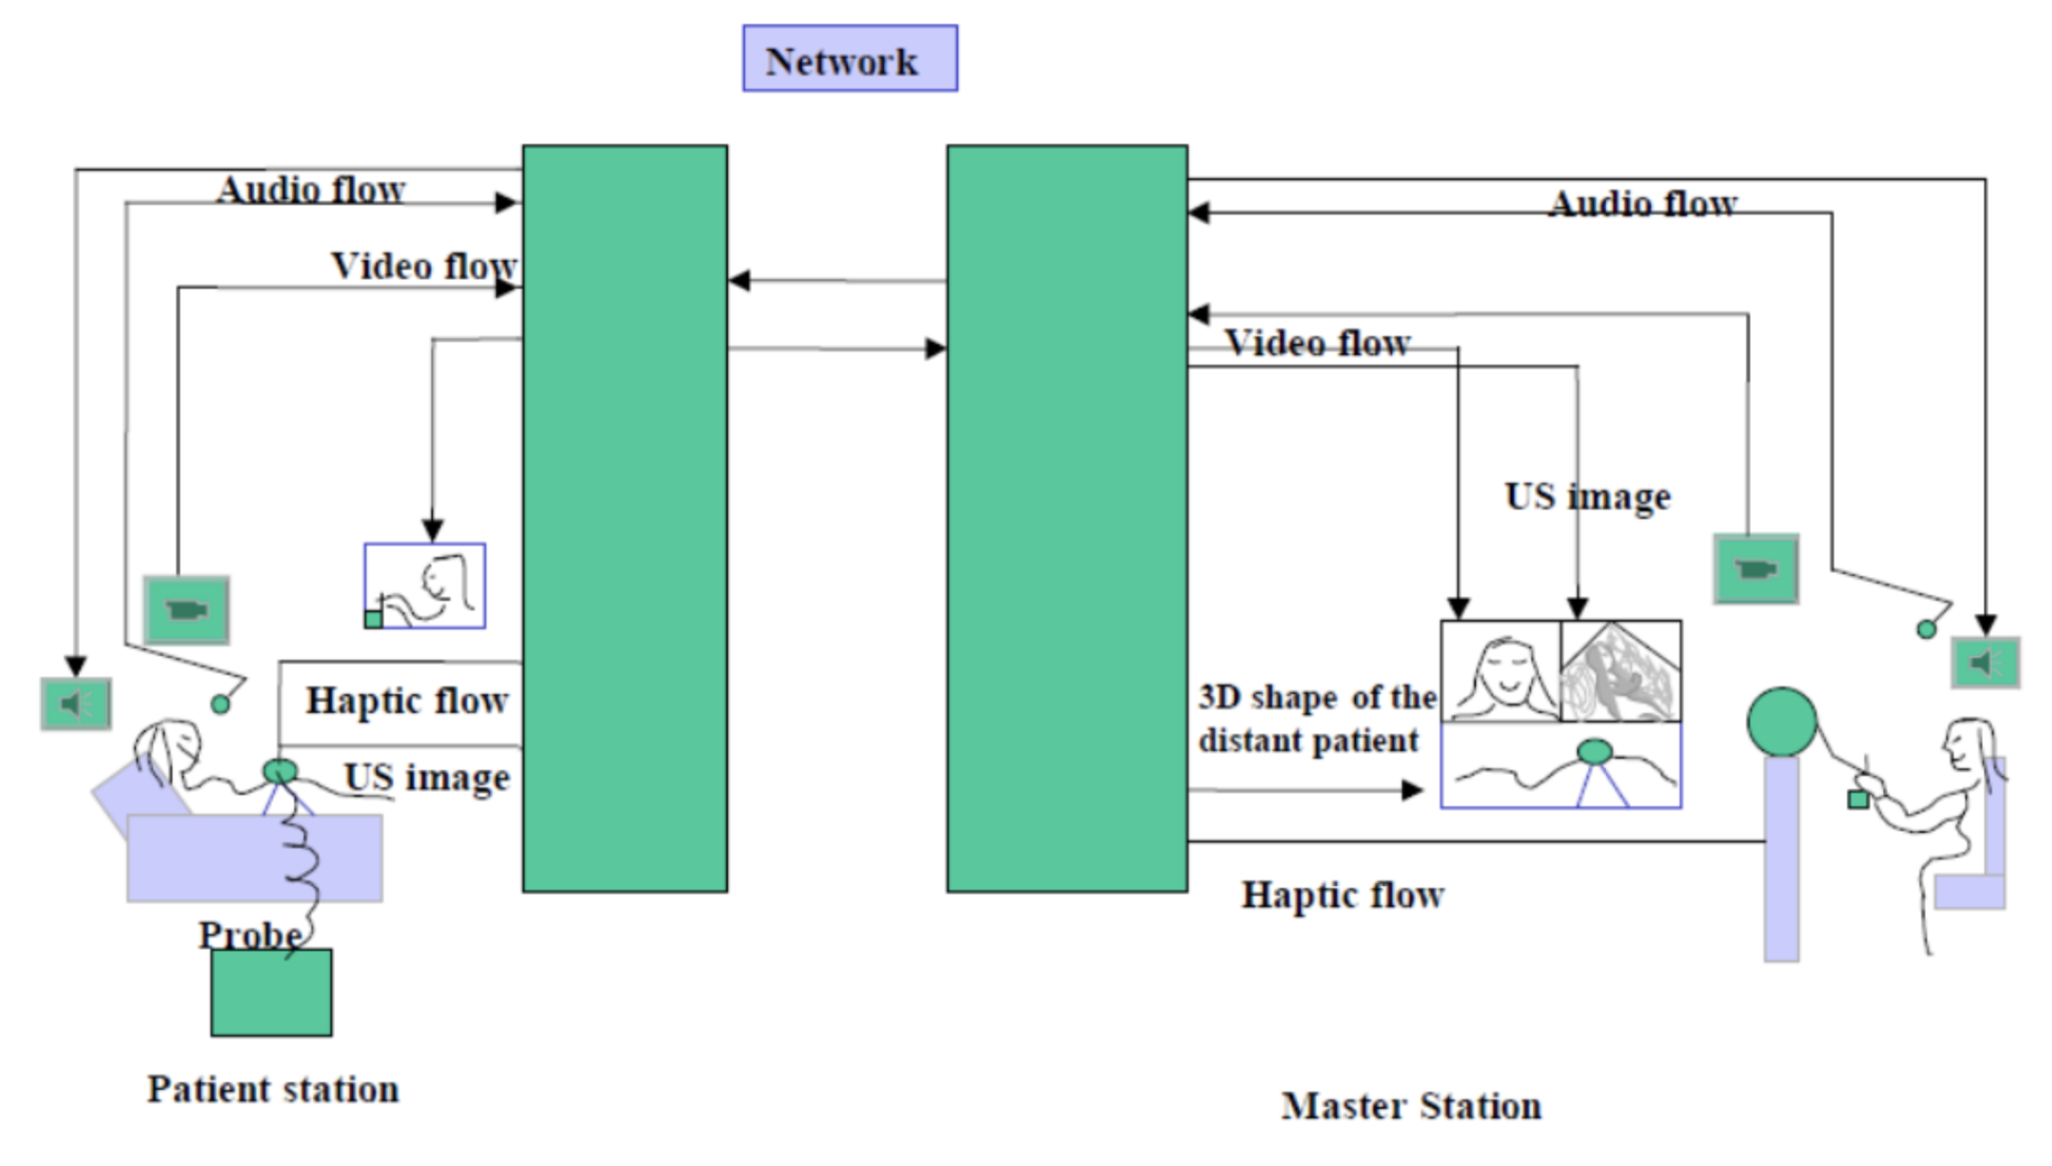
\includegraphics[width=0.7\textwidth]{TER.png}  
    \caption{TER architecture}
    \label{fig:ter}
\end{figure}


\subsection{The MELODY system}
The system operates under a long-distance paradigm, allowing for remote teleoperated ultrasound examinations, such as from a central hospital to a local facility or an isolated location. This approach offers several advantages, including increased access to specialized healthcare for remote communities and more cost-effective service delivery.
\\The system comprises three primary components: the expert system (master station), the patient system (slave station), and the communication link that facilitates data exchange between these two stations.

\begin{figure}[h]
    \centering
    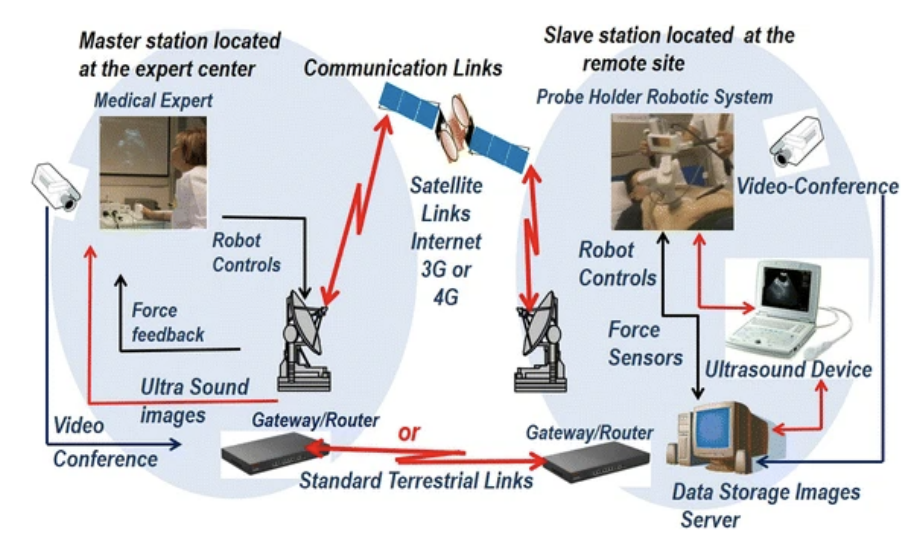
\includegraphics[width=0.7\textwidth]{MELODY.png}  
    \caption{The MELODY system}
    \label{fig:melody}
\end{figure}

\subsection{The OTELO system}
OTELO is a remotely operated system designed to perform reliable ultrasound imaging at a distant, isolated location without the need for a specialist clinician on-site. It is a mobile tele-echography solution utilizing an ultra-light robot, comprising three key components:

%\renewcommand{\labelitemi}{-}

\begin{itemize}
\item The expert site, where a doctor controls the positioning of the remote robot using a dedicated haptic probe. This probe mimics the feel and function of a traditional ultrasound probe, familiar to medical professionals, enhancing ergonomic comfort. The doctor also receives feedback on the contact force between the probe and the patient's skin, thanks to a force sensor located in the probe holder system.
\item The communication link, which can be either satellite or terrestrial, facilitates data transmission between the two locations.
The patient station, consisting of a lightweight 6-degree-of-freedom robotic system and its control unit. \item This robot manipulates the ultrasound probe in response to commands from the medical expert. It is maintained by a nurse or a non-specialist assistant, who positions and holds the robot on the patient’s skin under the guidance of the doctor via videoconference. The robot replicates the movements of the virtual probe on the real ultrasound probe.
\end{itemize}

\begin{figure}[h]
    \centering
    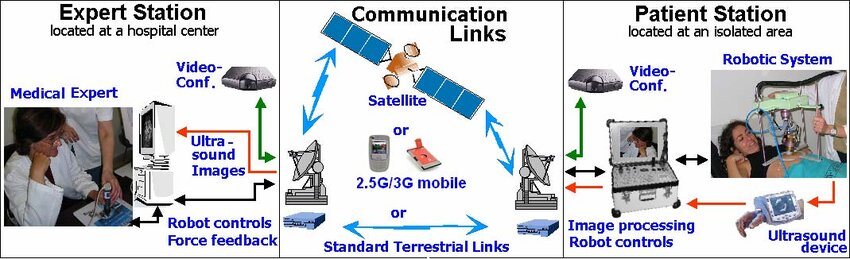
\includegraphics[width=0.7\textwidth]{OTELO.png}  
    \caption{The OTELO system}
    \label{fig:otelo}
\end{figure}


\begin{figure}[h]
    \centering
    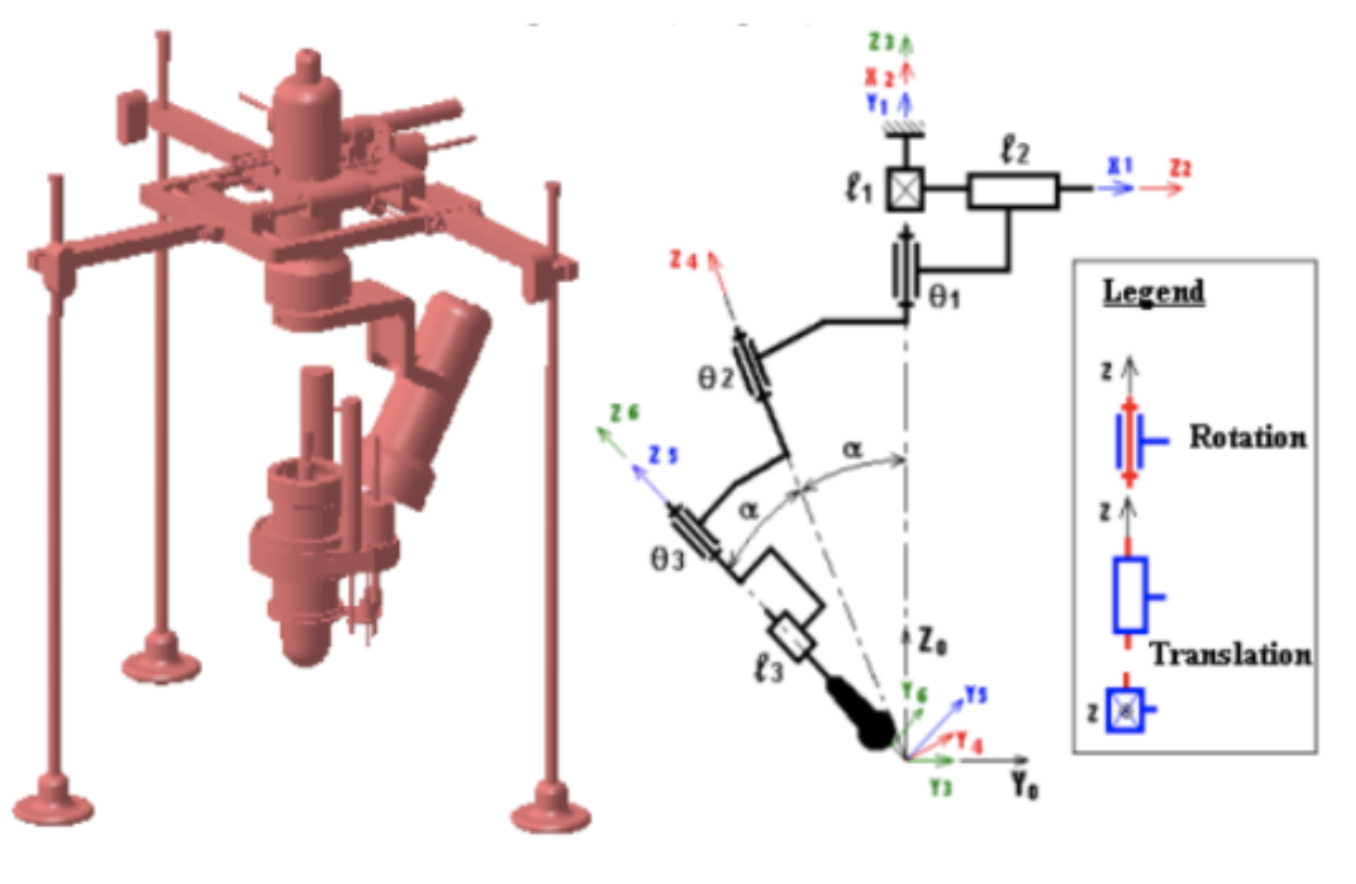
\includegraphics[width=0.5\textwidth]{OTELO_structure.png}  
    \caption{Mechanical structure of OTELO 1}
    \label{fig:otelo struc}
\end{figure}

\subsection{A previous project on related work}
Our colleagues implemented an impedance control system for a manipulator designed to perform a tele-echography task. The simulated manipulator is equipped with an ultrasound probe that interacts with an abdominal phantom. Starting from an initial position above the phantom, the probe approaches the abdomen perpendicularly and then slides across its surface while maintaining low contact forces.

\paragraph{Limitations:}
\begin{itemize}
\item The previous work did not fully achieve teleoperated motion under shared control, as it was limited to implementing pre-defined trajectories.
\item The robot's redundancy was not utilized to keep its structure at a safe distance from the patient, which is important for ensuring optimal safety during task execution.
\item No force/torque sensors were used in CoppeliaSim to measure the contact forces during the simulation.
\end{itemize}
\par



\section{Development}

\section{Conclusion}

\section{Future works}



\addcontentsline{toc}{section}{References}
\begin{thebibliography}{9}

\bibitem{Spong}
  M. Spong,
  \emph{“On the robust control of robot manipulators”},
   IEEE Trans . on Automatic Control, 37(11), 1782-1786, 1992.

\bibitem{Slotine}
  J.-J. E. Slotine, and W. Li,
  \emph{“On the adaptive control of robot manipulators”},
  Int. J. Robot. Research, vol. 6, no. 3, pp. 49-59, Fall 1987.
   
\bibitem{De Luca}
  A. De Luca,
  \emph{RobustControl},
 Block of slides 11 RobustControl of Robotics 2

\end{thebibliography}

\end{document}